\documentclass[11pt]{book}

\usepackage[width=7.0in, height=9.0in, top=1.0in, papersize={8.5in,11in}]{geometry}
\usepackage[pdftex]{graphicx}
%\usepackage{datetime}
\usepackage{anyfontsize}
\usepackage{t1enc}
\usepackage{verbatim}
\usepackage{algorithm}
\usepackage{algorithmic}
\usepackage{framed}
\usepackage{pdfpages}
\usepackage{listings}
\lstset{language=C}

\lstset{language=python,frame=ltrb,framesep=5pt,basicstyle=\normalsize,
 keywordstyle=\ttfamily\color{DarkRed},
%morecomment=[n][\textbf]{In\ [}{]\:},
%morecomment=[n][\textbf]{Out\ [}{]\:},
morecomment=[s][\color{blue}]{In\ [}{]\:},
morecomment=[s][\color{red}]{Out[}{]\:},
identifierstyle=\ttfamily\color{DarkBlue}\bfseries,
commentstyle=\color{DarkGreen},
stringstyle=\ttfamily,
showstringspaces=false,tabsize = 3}


\lstdefinelanguage{shell} {
commentstyle = \color{black},
keywordstyle = \color{black},
stringstyle = \color{black},
identifierstyle = \color{black},
morecomment=[s][\color{blue}]{In\ [}{]\:},
morecomment=[s][\color{red}]{Out[}{]\:},
 }

\pagestyle{empty}

\usepackage{helvet}
\renewcommand{\familydefault}{\sfdefault}

\begin{document}


\fontsize{16}{16}\selectfont Sprint Report \#1


\section{Team Members:}
Dicheng Wu
\\Marcus Berger\\
\textbf{Sponsor:}
\\Jeff McGough
\\

\section{Customer description}

\subsection{Description of sponsoring customer}
The sponsoring customer for this project is Dr. Jeff McGough a computer science professor at the South Dakota School of Mines and Technology and the vice president of the Academy of Dance Arts in Rapid City, South Dakota. Well not the sponsor of the project Dr. McGough's wife is also a key part of the customer base as the owner of the Academy. She and other dance school owner are the target group for this project. 

\subsection{Statement of customer's problem or goal for this project}
The customer wants a software that can run the day to day operations of a dance studio and also handle record keeping, billing, payroll, and other business operations
 
\subsection{Customer's Needs}
The customer needs us to develop a software solution which can run the dance studio in an effective manner. The product also needs to handle changing classes from year to year without needing to be updated. This means that the software needs to sync with multiple users, and handle new information such as class rosters, prices, clothing requirements for classes, changes in the employment roster, and many other changes that can occur in the running of a dance school.\\
This project as a whole needs to be an improvement on the current system in use by the customer and provide an easy and efficient way to run the clients business. 



\section{Overview of the project:}
The project consists of three major parts, Gui, database and back end code. For the Gui part, we are going to integrate everything into a small number of windows to eliminate the need for large numbers of window like the current product in use at the academy. and, thus, users can manipulate it very straightforwardly. For database part, we are going to build a database which stores students, employees, classes, billing, and other information needed for the academy to function as a business. For the code back end, we are going to develop it on using Python and PyQt with a primary focus on Mac but with cross platform compatibles. 

\section{Project Environment:}

\subsection{Project boundaries}
The boundaries of this project would be the Academy of Dance Arts in Rapid City. The product could be used by other dance schools in the future but they are out of the scope of this projects development 

\subsection{Project context}
The context of this project is only to develop a better software solution to the current software in use at the Academy of Dance Arts in Rapid City, South Dakota, so they can run their school in a more efficient manner. While the project is open source it is not the intention of this team to develop an all purpose solution for all the dance schools around the country. This project is tailored to the needs of the Academy of Dance Arts.


\section{Project deliverables of Sprint 1:}

\begin{enumerate}
\item The research into program languages, database and Gui frameworks and architectures for the DanceSoft project.
\item Final decision on frameworks and architectures for the DanceSoft project.
\item User Stories and Product Backlogs for the project.
\item Creating a very simple Qt window.
\end{enumerate}

\section{User Stories}

After the requirement for the project were laid out the team created the user stories based on those requirement. The user stories the team came up with fallow:

\begin{enumerate}
  \item As a user i want to adjust students payment models
  \item As the owner I would like to see automatic database backups.
  \item As a student I would like to be able to register online (with special app). Classes must be approved before added.
  \item As a student I would like to be able to search clothing requirements.
  \item As a student I would like to know my billing.
  \item As the owner I would like to indicate clothing requirements per class.
  \item As a studio person, I would like to be able to add students to classes.
  \item  As a student, teacher etc, I would like to be able to look up a students class list.
  \item As the teacher I would like to get a class role for each class.
  \item Given a class list, I would like to get an invoice of the tuition due.
  \item Studio would like to track payments and estimate remainder due.  I would like to generate an invoice for this amount.
  \item As a student I would like to be able to register online (with special app).   Classes must be approved before added.
  \item As a student I would like to know my billing.
  \item As the owner I would like to track teacher hours and compute payroll.
  \item As the owner I would like to indicate clothing requirements per class.
  \item As a student I would like to be able to search clothing requirements.
  \item As the owner I would like to see automatic database backups.
\end{enumerate}

\section{Product Backlog:}

From the above user stories the team produced the fallowing product backlog. The parts are not in the order of execution. More thing will be add or removed to this in the future as the software develops.

\begin{enumerate}
\item Create the database tables
\item Create database backup system
\item Create online register page and approval system
\item create clothing requirement update function, and add clothing function for teachers and admin
\item create clothing viewer function for students
\item create dynamic billing algorithms (expand on later sprint)
\item create page for tuition calculation and viewing by students
\item Add and subtract students from a class
\item Create dynamic Queries to produce class attendance list
\item Hour tracker for teachers and payroll calculation algorithm (expanded later)
\item Using dynaminc DNS service to set up Linux Box
\item Encrypt data that store in the database
\item retrieve data from database to produce a invoice for payroll
\item queries in database to retrieve student information
\item Create ability for employee to look up and modify student registration info
\item Query database to produce class role sheet
\item Query database to produce employee information
\item create permission assignment system
\item handle billing info (expand later)
\item Create dynamic algorithm for payment model creation and calculation. 
\item Algorithm for payment tracking and remainder calculation, and query database to produce invoice.
\item Query and insert information needed to create and new class and produce a results page.
\item Create update query to assign teachers to a class
\end{enumerate}

\begin{figure}
\caption{DanceSoft Trello Board}
\centering
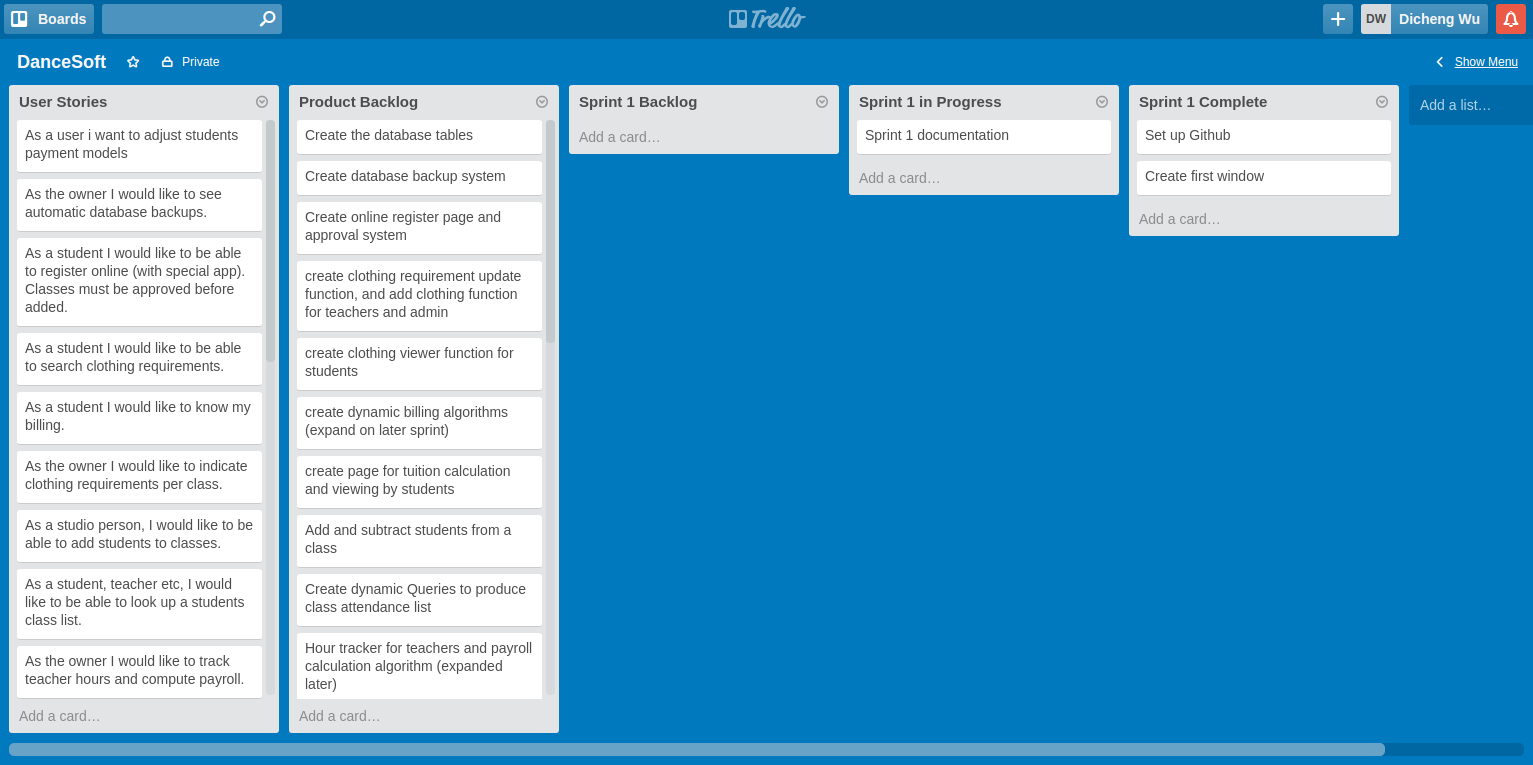
\includegraphics[width=0.5\textwidth]{d1}
\end{figure}



\subsection{Sprint 1 Backlog:}

\begin{enumerate}
\item Set up Github
\item Design Research
\item Design Decision
\item Create first window
\item Sprint 1 documentation
\item Sprint 1 Review
\item Continuing practice with QT

\end{enumerate}

\section{Research}

\subsection{Database Research}

\subsubsection{SQL VS NonSQL:}
SQL is designed for fixing data structure and the scale of amount of data in database should be medium size otherwise with it growing big the database will drop down its speed. NonSQL is designed for frequent changing data structure and the scale of amount of data in database does not affect the performance of the database a lot. The SQL database is stable and however the NonSQL is constantly suffering failovers. The database aims to store employees and students and classes information and the size of students less than 4000 and the size of employees less than 10. The structure of data is stable, by considering all those facts above, we decide to use SQL database.\\

\textbf{The different SQL Databases:}\\
For this part, we think of using Mysql, SqLite, Mssql. Mysql is a free software and widely used in different fields. It has a very good portability and can runs over different OS systems and aims for small size of data. Also our experience is more focused in MySQL, and the feature set for SQL in MySQL fits within the scope of the project, for these reasons we choose MySQL as the database frame work.

\subsection{Storage Options:}
For this part, We considered three options, local, cloud, mixed. Since the database is accessed by different devices and the internet in the Academy is not stable, we decide to use mixed storage schema either Amazon AWS plus a local database or a Linux box plus a local database. After researching Amazon AWS, it does not support storing images and videos which the Academy may require in the future, therefore   due to some inconsistency in the internet and the current and possible future needs of the Academy we decided to go with a local Linux box and database.\\

\subsection{Languages}
Since the Academy is currently running a Mac system the first langauge idea was objective-C. Recently though Apple released a programming language update called Swift. Due to our teams inexperience with Mac and the possibility of the dance academy being sold in the future we were faced with a choise, between Python or Swift. Swift is a c++ like language which stuck out as a possible jumping off point for us. However as we researched it became clear that swift would have a high ramp up time and learning curve. On top of this as novices to the Mac development environment we would spend a large amount of time just trying to figure out the system. As far as pluses for Swift the language has all the functionally of objective-C plus things added to make the language better, overall reception for the language within the Mac community have been positive. The language itself is designed with porting to IOS in mind which would make a mobile transition more likely. The language would use Cocco as a GUI environment which is also relatively well revived by OSX developers, ut again ramp up for our team would be high.

The language competing with Swift in our discussions was Python. Python has the upside of being a language the team is more experienced in. Also the client Dr. McGough knows Python so any updates would be easier for him to do. Python is also a cross platform language which allows the team to produce working code for Mac, Windows, and Linux at the same time and on any operating system. This means the the team can develop on Windows or Linux, development environments we are more familiar with, and have the code work on Mac. Also development in Python means that if the academy was ever sold to a Windows user the product would still work. Another advantage we discovered to python is the academic and career experience it provide since in our research for the SD Mines career fair we discovered that many companies use Python and more than expected would like QT experience. Lastly the Python community is larger and can more readily provide assistance if needed through websites and research.

So overall while Python is not Mac native it provides more viable reasons for use in our teams eyes. That is not to say we don't believe Swift is a good choice, Swift is a completely viable choice for a product like this it is just not the best for the exact situation the team is in. So we have decided to create the  Academy of Dance Arts Software in Python using PyQt as a GUI. 

\subsection{Final Framework Decision}
Language: Python\\
Gui: PyQt\\
Database: Mysql\\

\section{Foreseeable issues}
As of the sprint 1 review, possibly issues could include database encryption and synchronization, team learning curve of Qt.


\end{document}